\documentclass{article}
\usepackage{graphicx} % Required for inserting images
\usepackage{float} % For figures placement
\usepackage{fancyvrb} % for \Verb
\usepackage[a4paper, margin=2.5cm]{geometry}
\usepackage{karnaugh-map} % Tableau de Karnaugh
% Subfigures
\usepackage{caption}
\usepackage{subcaption}

\usepackage{amsmath}
\usepackage{emoji}

\usepackage{enumitem}

\usepackage[hidelinks]{hyperref}




\usepackage{setspace} % to change line spacing
\renewcommand{\baselinestretch}{1.5} 


\setlength{\parskip}{\baselineskip}%
\setlength{\parindent}{0pt}%

\begin{document}

\makeatletter
\begin{titlepage}
\begin{center}
    

\includegraphics[width=7cm]{assets/LogoCN_Q.png}
\\
\textbf{\large{Centrale Nantes}}
\\[2cm]

\textbf{\large{MAC : $1^{st}$ Lab's Report \\
Build an 8-bit ALU with Logisim}}
\\[14pt]
$1^{st}$ year Embedded Systems Engineering
\\[2cm]


\vfill

\textbf{By} \\
EL KHAYDER Zakaria \\
SAOUTI Rayan
\\[1cm]

\textbf{Professor} \\
BRIDAY Mikael
\\[3cm]


October 22, 2023 \\ [12pt]

Session \\
2023-2024 \\[12pt]
\small{Made with \LaTeX}
\end{center}
\end{titlepage}
\makeatother

\pagebreak

\setcounter{page}{1}
\pagenumbering{Roman}

\clearpage
\addcontentsline{toc}{section}{Contents}
\tableofcontents

\clearpage
\addcontentsline{toc}{section}{List of Figures}
\listoffigures
\addcontentsline{toc}{section}{Table of Tables}
\listoftables

\clearpage

\setcounter{page}{1}
\pagenumbering{arabic}

\section{Adder}

\subsection{1-Bit Adder}

\subsubsection{Truth Table}

\begin{table}[H]
    \centering
    \begin{tabular}{|c|c|c||c|c|} \hline 
         $c_n$&  $a_n$&  $b_n$&  $c_{n+1}$& $s_n$\\ \hline \hline 
         0&  0&  0&  0& 0\\ \hline
         0&  0&  1&  0& 1\\ \hline 
         0&  1&  0&  0& 1\\ \hline 
         0&  1&  1&  1& 0\\ \hline 
         1&  0&  0&  0& 1\\ \hline 
         1&  0&  1&  1& 0\\ \hline 
         1&  1&  0&  1& 0\\ \hline 
         1&  1&  1&  1& 1\\ \hline
    \end{tabular}
    \caption{1-Bit Adder Truth Table}
    \label{tab:1Bit Adder Truth Table}
\end{table}

{
\small
\begin{description}
  \item[$a_n$:] Input A (1-Bit).
  \item[$b_n$:] Input B (1-Bit).
  \item[$c_n$:] The Carry from the previous stage (1-Bit).
  \item[$s_n$:] This stage's result (1-Bit).
  \item[$c_{n+1}$:] This stage's Carry (to be used in the next stage) (1-Bit).
\end{description}
}

\subsubsection{Karnaugh Map}
\begin{figure}[H]
    \centering
    
    \begin{subfigure}[b]{0.49\textwidth}
        \centering
        \begin{karnaugh-map}[4][2][1][$b_n$][$a_n$][$c_n$]
            \implicant{1}{1}
            \implicant{2}{2}
            \implicant{4}{4}
            \implicant{7}{7}
            \minterms{1, 2, 4, 7} % Ones
            \maxterms{0, 3, 5, 6} % Zeros
        \end{karnaugh-map}
        \\[-18pt]
        \subcaption{$s_n$}
     \end{subfigure}
     \hfill
     \begin{subfigure}[b]{0.49\textwidth}
        \centering
        \begin{karnaugh-map}[4][2][1][$b_n$][$a_n$][$c_n$]
            \implicant{3}{7}
            \implicant{5}{7}
            \implicant{7}{6}
            \minterms{3, 5, 6, 7} % Ones
            \maxterms{0, 1, 2, 4} % Zeros
        \end{karnaugh-map}
        \\[-18pt]
        \subcaption[labelformat=empty]{$c_{n+1}$}
     \end{subfigure}
     
    \caption{1-Bit Adder Karnaugh Map}
    \label{fig:1Bit Adder Karnaugh Map}
\end{figure}


\subsubsection{Equations}
Using the two Karnaugh Maps extracted from the truth table above, we can find the two simplified equations for $s_n$ and $c_{n+1}$.
$$
c_n = a_n \cdot b_n + a_n \cdot c_n + b_n \cdot c_n
$$
We notice that the 4 implicants in $s_n$ are made up of only one single bit each, which does not simplify any of the input, making each group equation depend on all three inputs.
% \vphantom b in the equation makes the height of the character the same so the bar is on the same level
$$
s_n = \overline{a_n \vphantom b} \cdot b_n \cdot \overline{c_n \vphantom b} +  a_n \cdot \overline{b_n} \cdot \overline{c_n \vphantom b} + \overline{a_n \vphantom b} \cdot \overline{b_n} \cdot c_n + a_n \cdot b_n \cdot c_n
$$

However, given the definition of XOR:
$ a \oplus b = \overline{a \vphantom b} \cdot b + a \cdot \overline{b} $, we can see that the previous equation can be simplified, and with some experimentation, we found that $s_n$ can be written as
$$s_n = (a_n \oplus b_n) \oplus c_n$$


We are not sure how this could be reached, as the first equation contains both XOR and XAND gates, and they are kinda confusing to deal with, nevertheless, this worked \emoji{smile}

\subsubsection{Circuit}
We won't be pointlessly explaining how to implement the circuit in \verb|Logisim Evolution| (connections, circuits' placement), as this is not the point of the Lab Session, so we will insert screenshots of the circuits directly.

\begin{figure}[H]
    \centering
    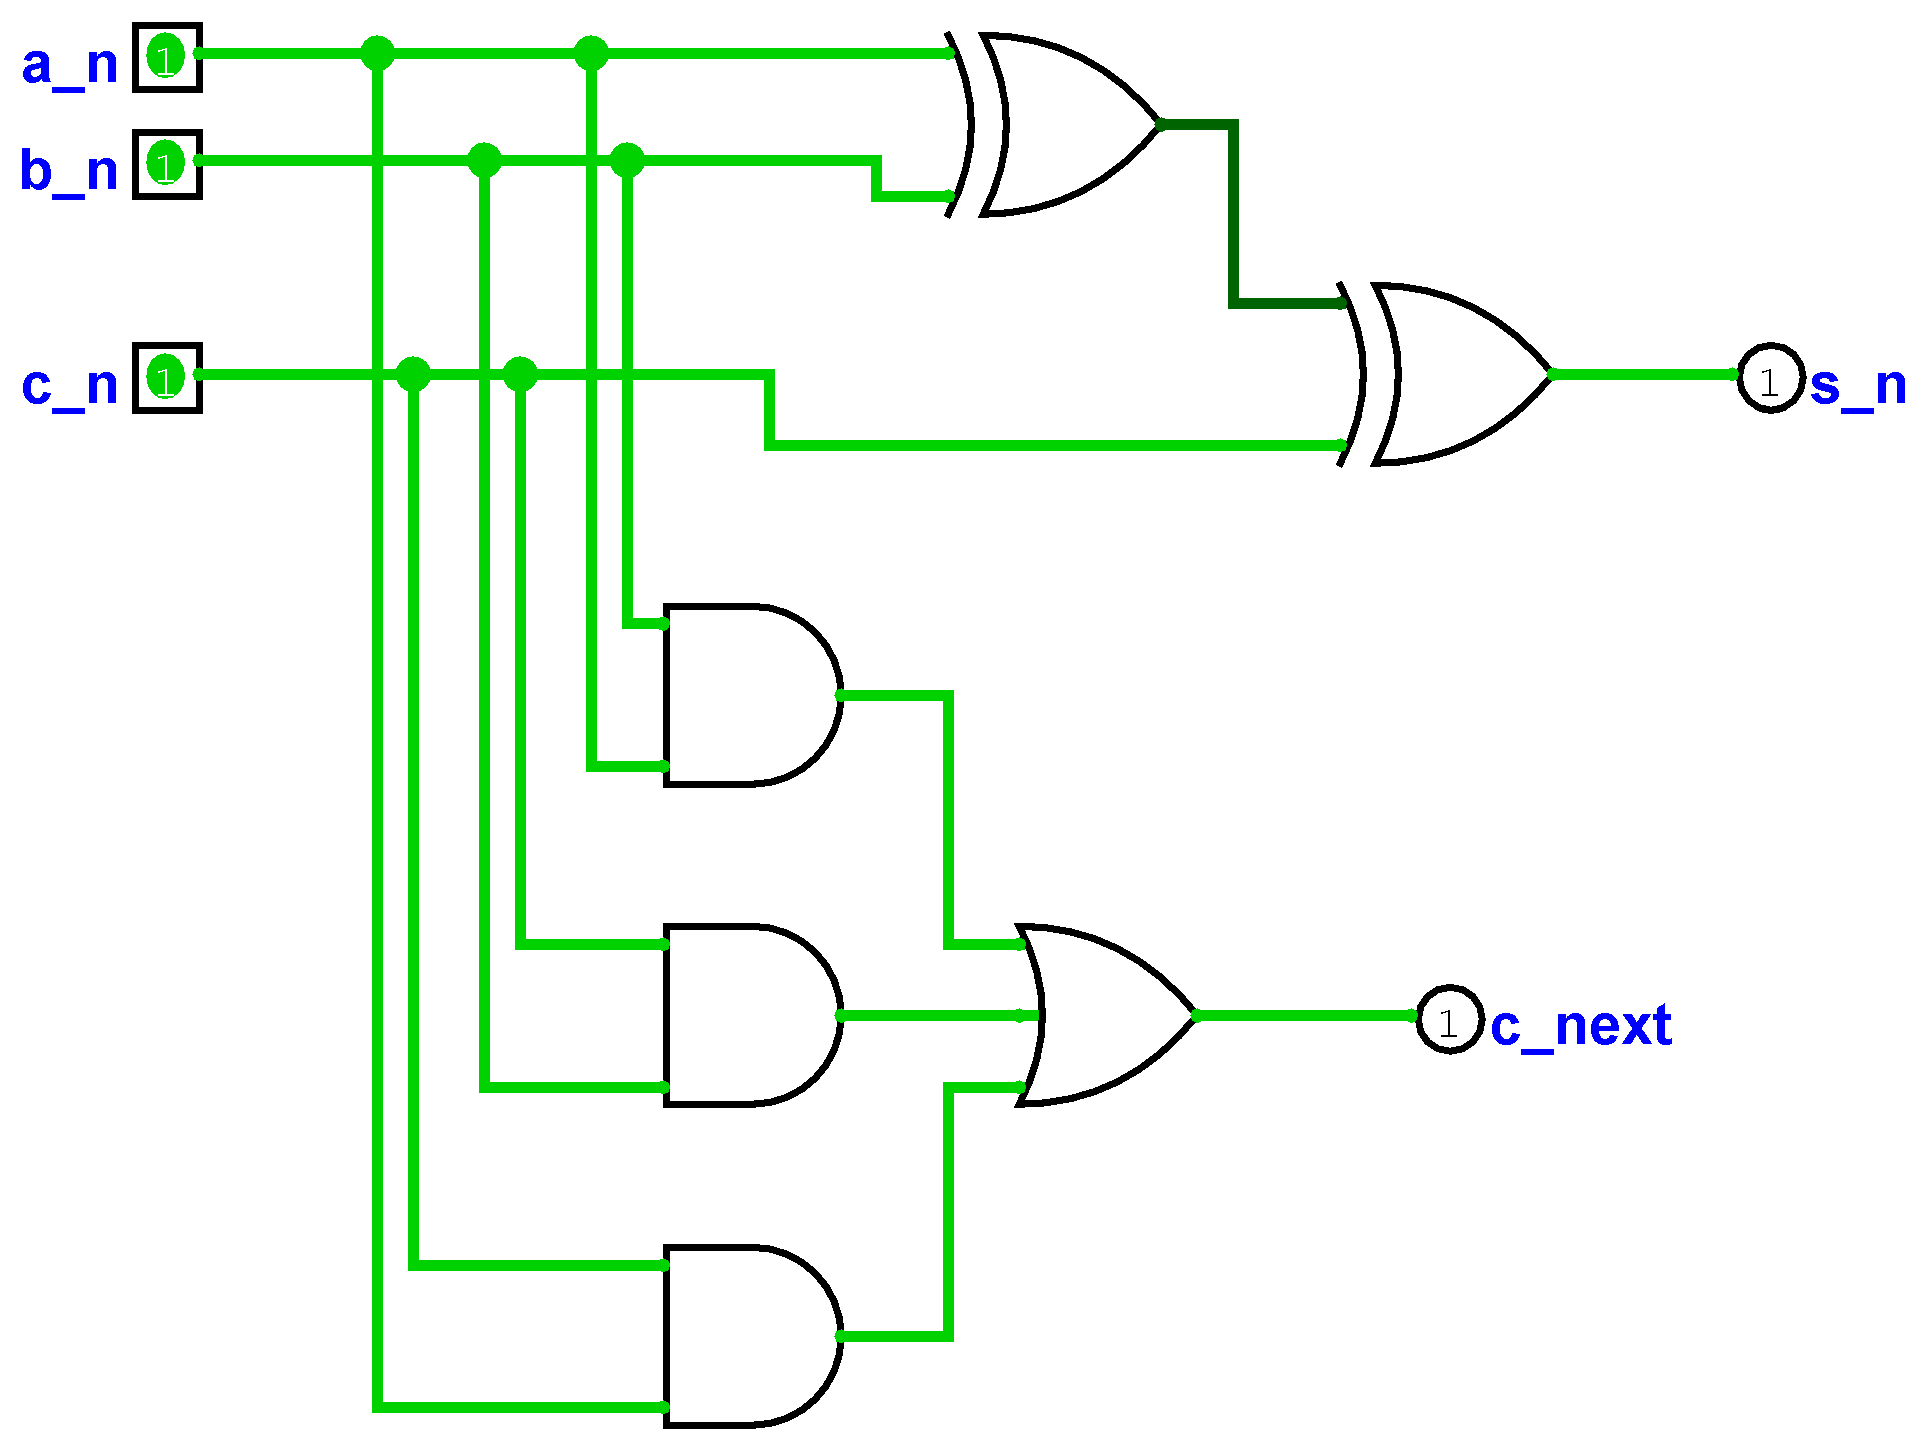
\includegraphics[width=.8\textwidth]{circuits/OneBitAdder.png}
    \caption{1-Bit Adder Circuit}
\end{figure}

\subsection{8-Bit Ripple-Carry Adder}

\subsubsection{Logic}
An 8-bit binary adder can be simply achieved by chaining 8 1-bit adders and connecting each $c_{n+1}$ to $c_n$ of the next stage (as the name of the circuit suggests). \\
This actually can be done for any size $n$.

\subsubsection{Circuit}
To simplify the usage, and make the circuit more concise, we used Logisim's built-in splitters and bus input/output.

\begin{figure}[H]
    \centering
    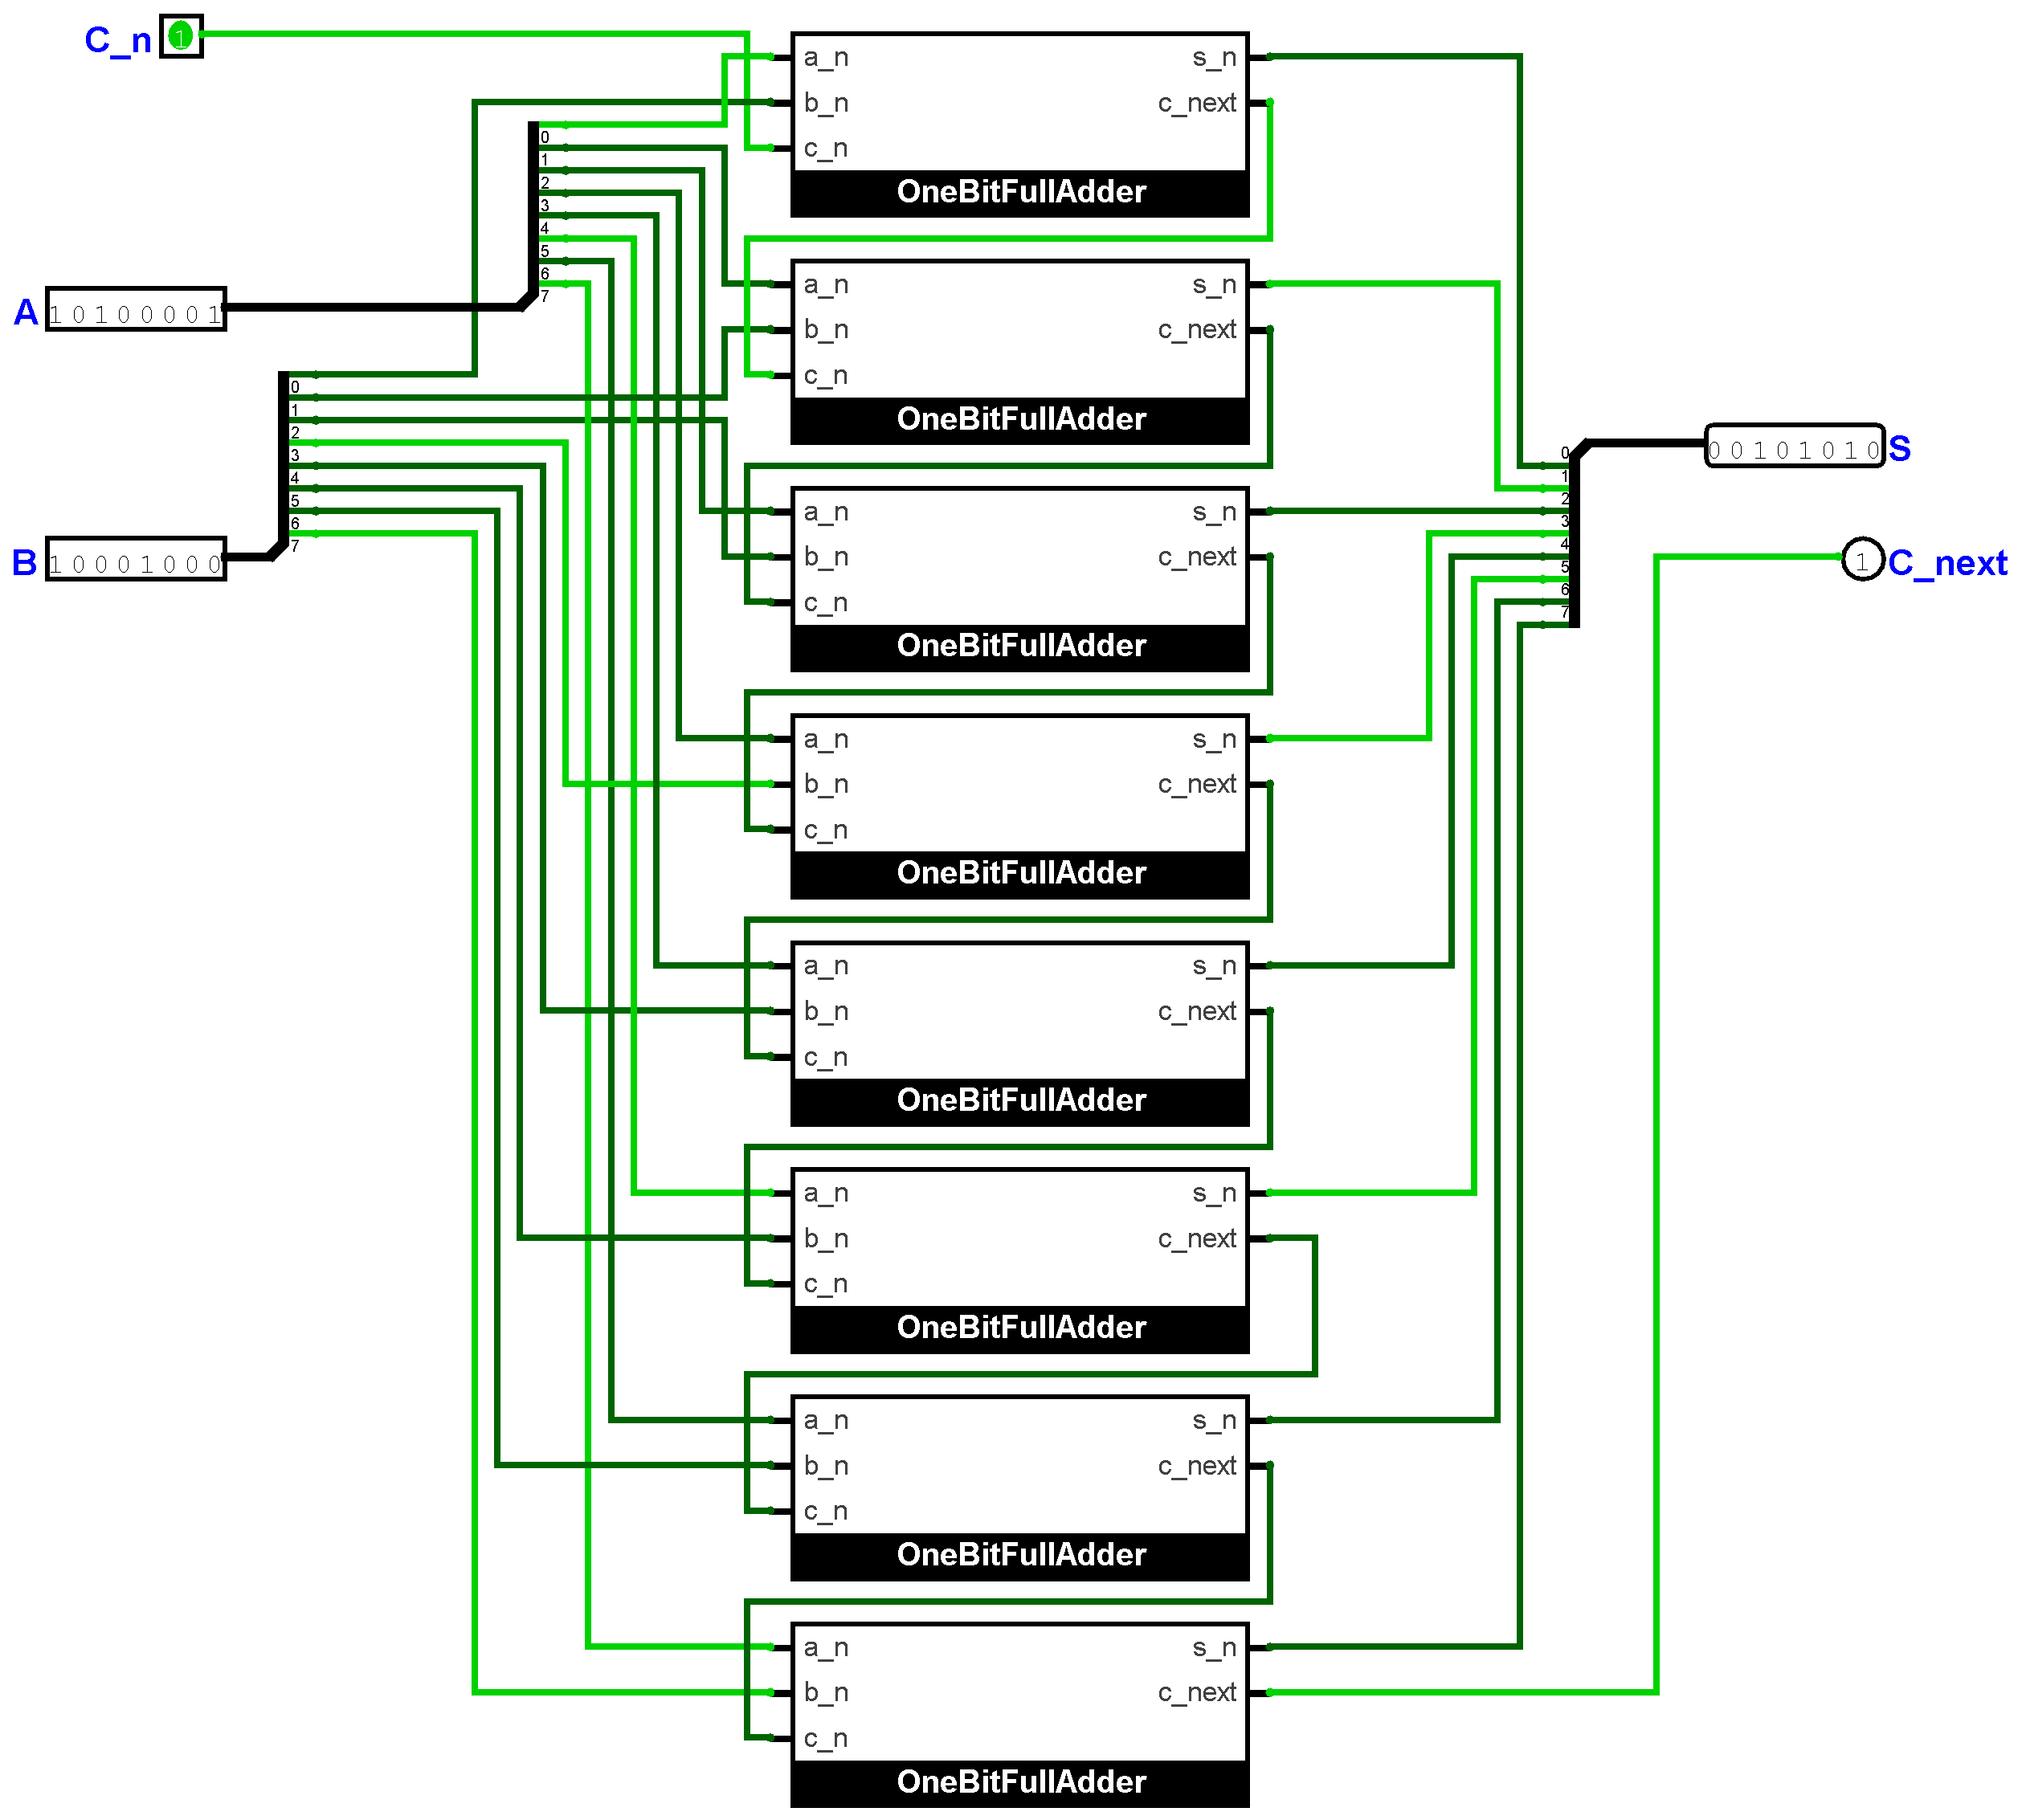
\includegraphics[width=\textwidth]{circuits/EightBitAdder.png}
    \caption{8 Bits Ripple-Carry Adder Circuit}
\end{figure}

The circuit shows the correct result of the addition of
$$
1010\:0001\;(161) + 1000\:1000\;(136) + 1\;(1) = 1\:0010\:1010\;(298)
$$
The result is on 9 bits, with the Carry being the MSB.

\section{ALU}

\subsection{Operations}

\subsubsection{Output Control / Selected Operation}
Given that the ALU should execute many operations, we need a way to control which of the operations to execute. This is done through the 3-bit \verb|OP| input, which allows us to select between $2^3 = 8$ different operations, mapped as the following:
\begin{enumerate}[start=0, before=\small, after=\normalsize, itemsep=2pt, parsep=0pt]
    \item addition
    \item subtraction
    \item and
    \item or
    \item not: \textasciitilde{} a (Changed to arithmetic shift right later-on)
    \item xor
    \item shift left a << b
    \item shift right: a >> b
\end{enumerate}

We used an 8 to 1 Multiplexer (provided by Logisim) to easily control the selected output, with the selection bus being coded on 3-bits (hence the 8 inputs) and each of the inputs and the output being an 8-bit data bus.

We used Tunnels instead of wiring everything to make the circuit cleaner and less crowded, and to avoid dumb wiring mistakes.

\begin{figure}[H]
    \centering
    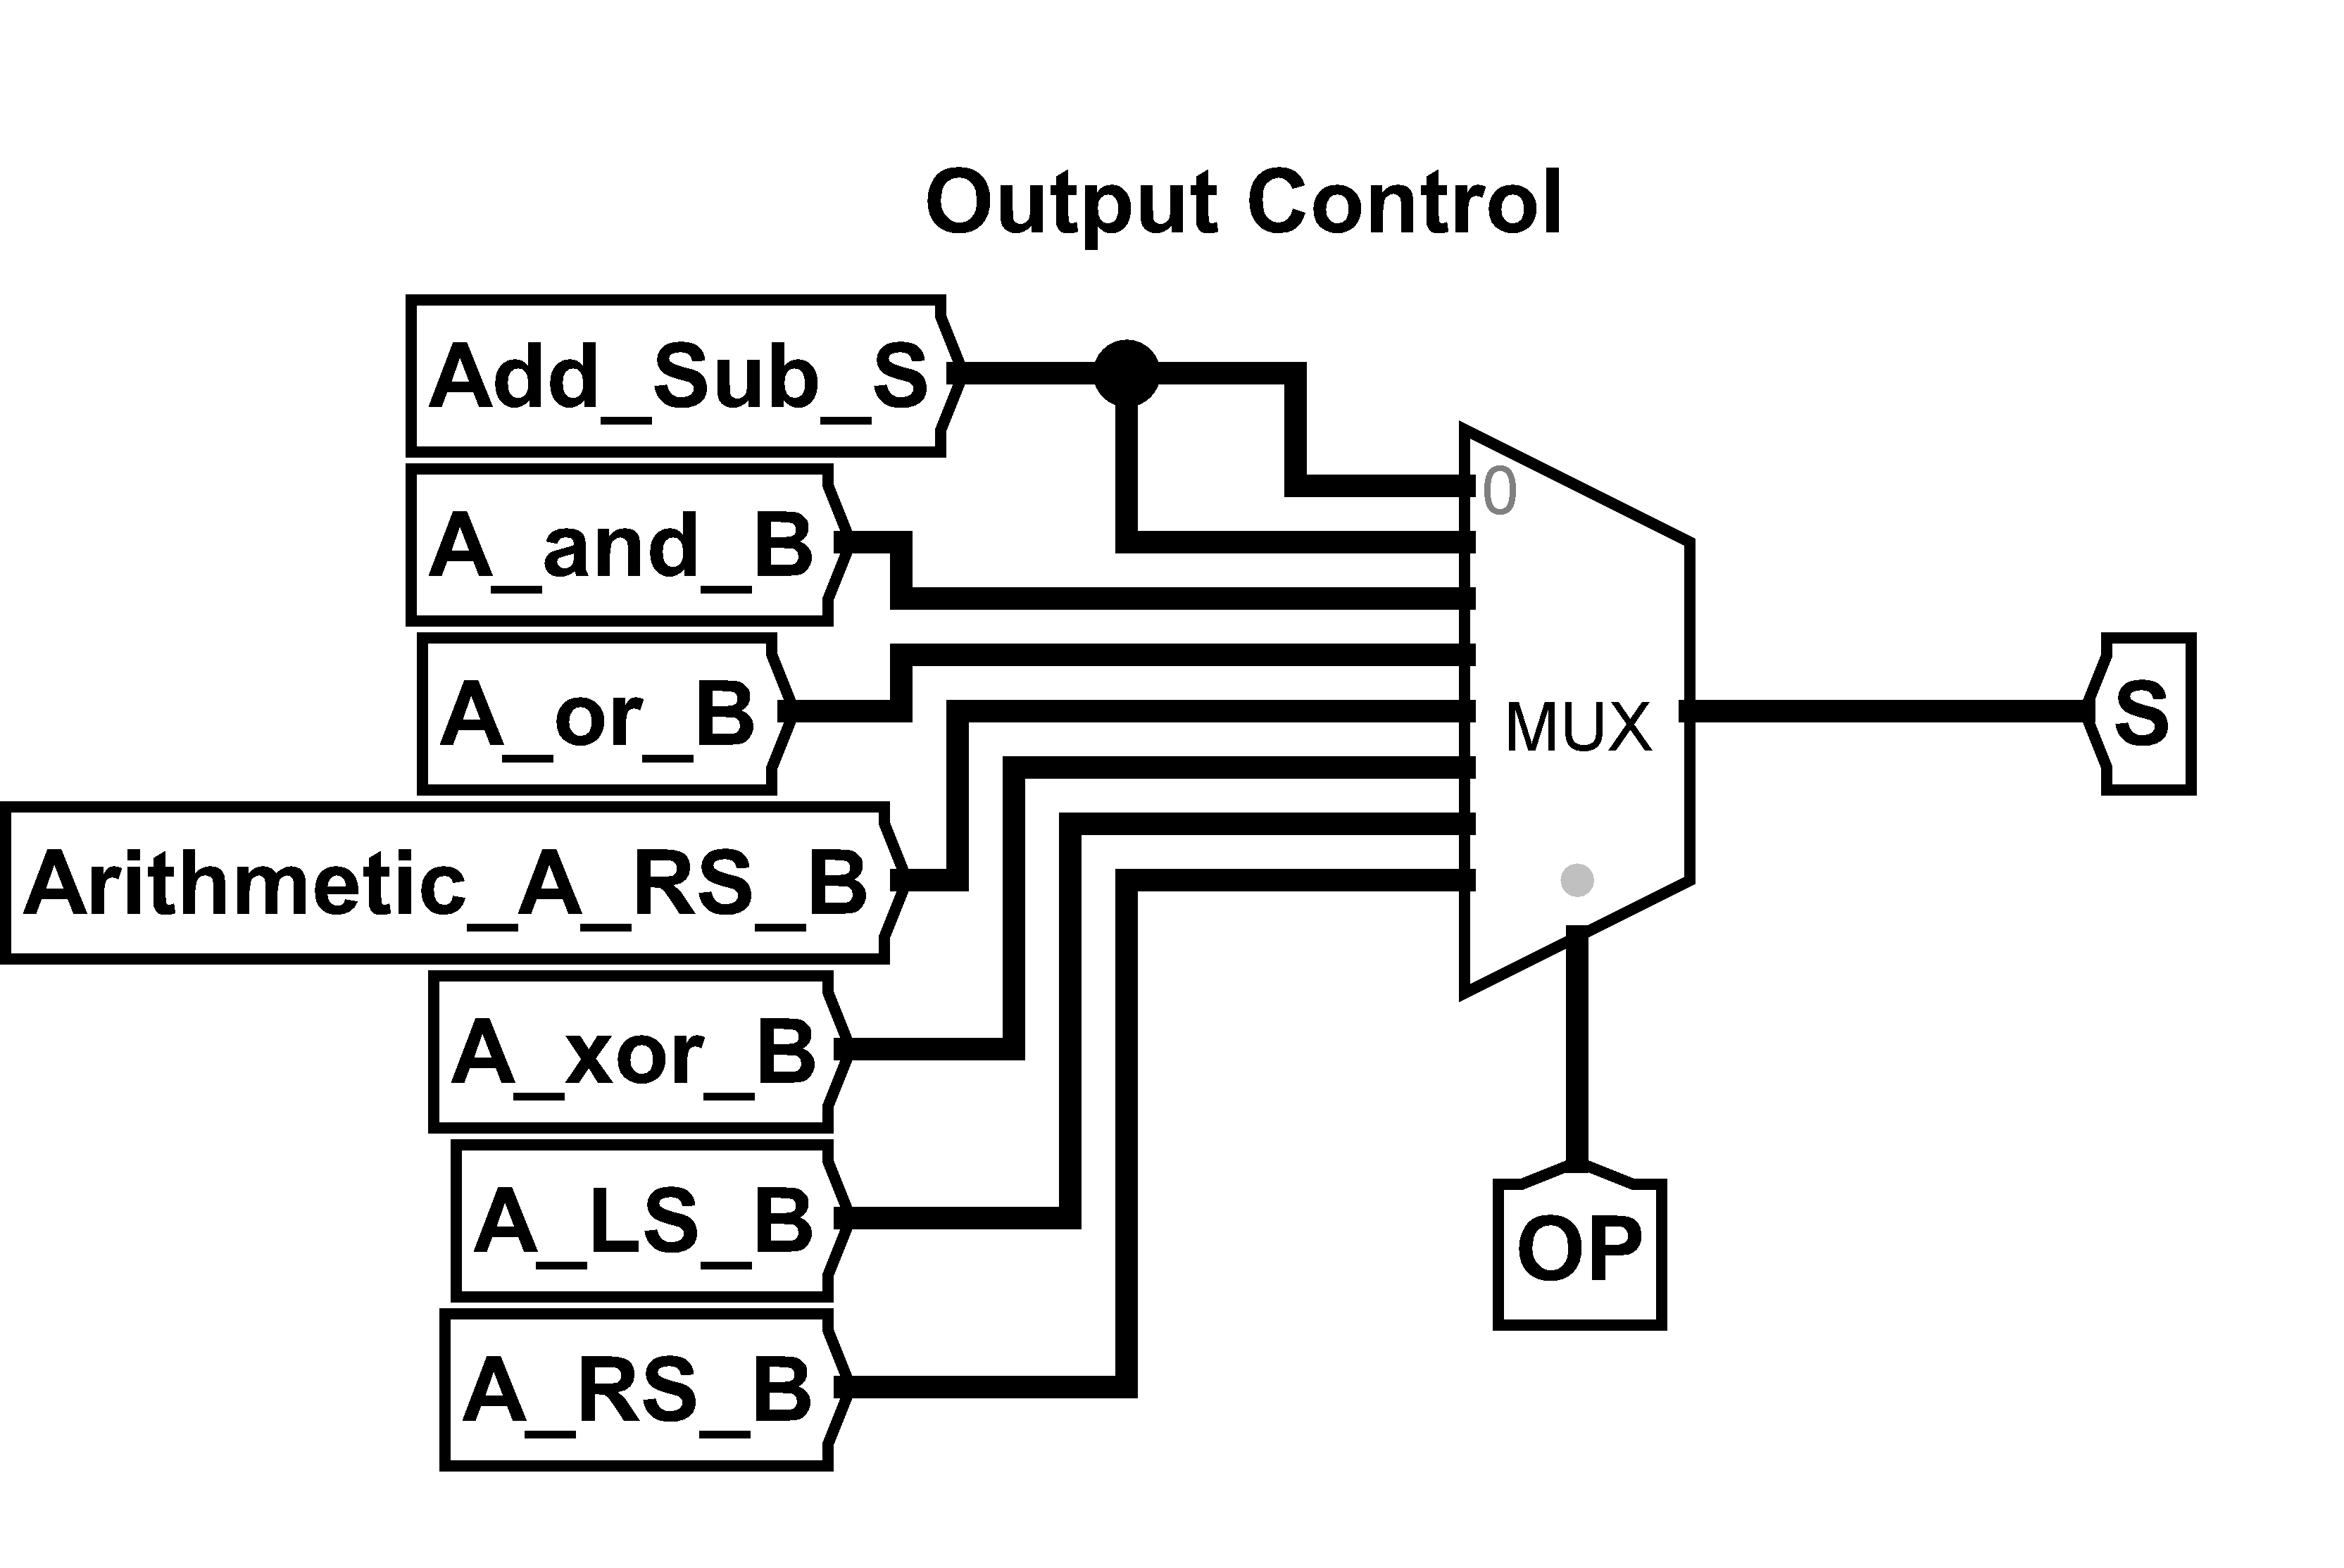
\includegraphics[width=.7\textwidth]{circuits/OutputControl.png}
    \caption{ALU Output Control}
\end{figure}

You notice that instead of having two tickets for both addition and subtraction, we have only one for both, connected to the two first inputs of the multiplexer. We will come back to this in the subtraction paragraph.\\
Also, the \verb|not| is already not there, as when this image was exported, we have already replaced it with the arithmetic right shift.

\subsubsection{Addition}

Implementing Addition is very straightforward, as we already have built an 8-bit adder, only left to connect the inputs and output to their proper correspondence.

\begin{figure}[H]
    \centering
    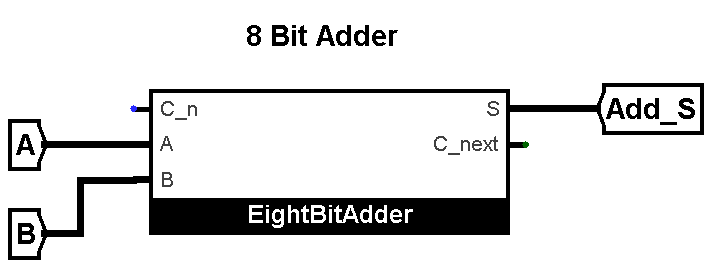
\includegraphics[width=.6\textwidth]{circuits/Add.png}
    \caption{ALU Adder}
\end{figure}

Nevertheless, this circuit will be soon changed when we implement the subtraction.

\subsubsection{Subtraction}

With some $6^{th}$ grade's math knowledge, we can deduct that $a - b = a + (-b)$, and with that, we can use the same 8-bit adder that we have built before to do the subtraction, the only thing left is inverting the sign of $b$. \\
We will be using 2's complement to represent negative numbers in our binary system, so $-b = \textasciitilde{}b + 1$.

Our first solution, involved first inverting $B$, then adding 1, and only then summing it with $A$.

\begin{figure}[H]
    \centering
    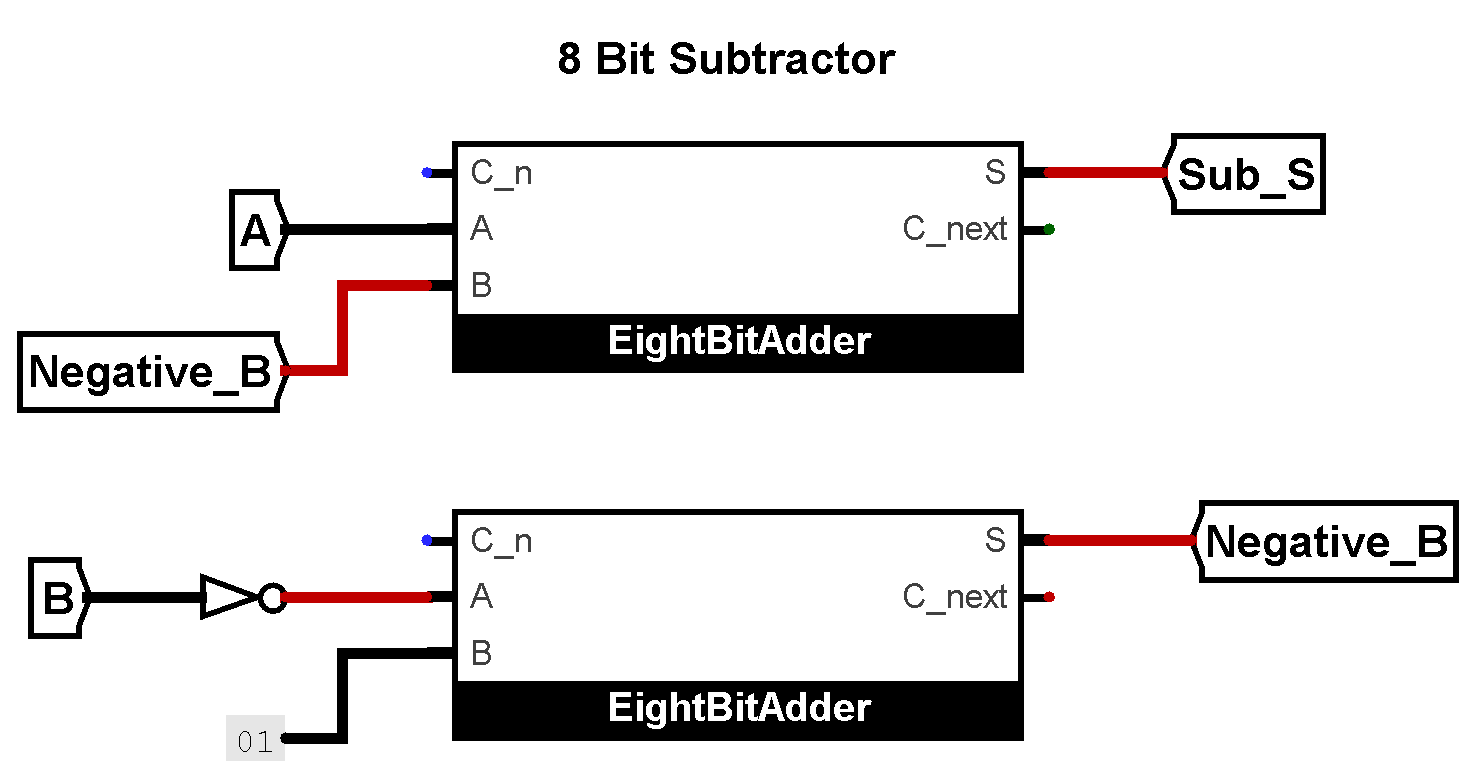
\includegraphics[width=.7\textwidth]{circuits/Subtractor_StupidWay.png}
    \caption{ALU Subtractor - With two adders}
\end{figure}

This solution works, however, we use two 8-bit adders to achieve this, and that is a waste of components since we can use the $C_n$ input for the $+ 1$ in our 2's complement equation, therefore reducing our subtractor to half its size.

\begin{figure}[H]
    \centering
    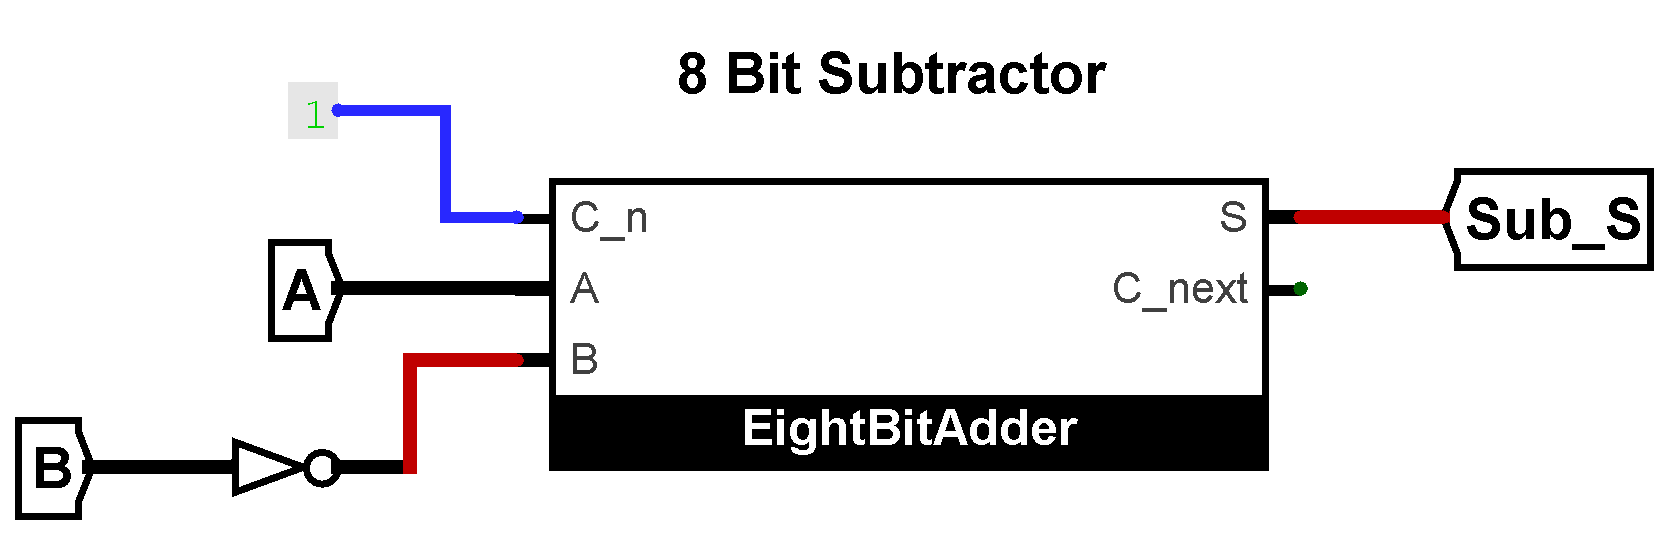
\includegraphics[width=.7\textwidth]{circuits/Subtractor_LessStupidWay.png}
    \caption{ALU Subtractor - With one adder}
\end{figure}

This is a more optimized solution for our subtractor, but let's not forget that we already have an 8-bit adder in our ALU, wouldn't be great to use it for both addition and subtraction? \textbf{Well, WE CAN!}

\subsubsection{Adder/Subtractor}
 As hinted above, we can use a single adder to do both addition and subtraction in our ALU, reducing the used number of adders by two-thirds, from 3 to 1.

 We can check if the \verb|OP| input is set to subtraction ($=1$), if so, we can run invert the $B$ input and set $C_n = 1$ of our adder to make it calculate $S = A + \textasciitilde{}B + 1 = A + (\textasciitilde{}B + 1) = S = A + (-B) = A - B$, otherwise we can run normal addition of $A$ and $B$. \\
 We will have a single output for both addition and subtraction, that we connect to both addition and subtraction result inputs on our Output Control Multiplexer (exactly what we have in the image before).

 For OP to be set to Subtraction ($=1$), $OP = 001_{(2)} \Rightarrow{} \overline{OP_2} \cdot \overline{OP_1} \cdot OP_0$.\\
 We can add a simple AND gate for the check.

 \begin{figure}[H]
     \centering
     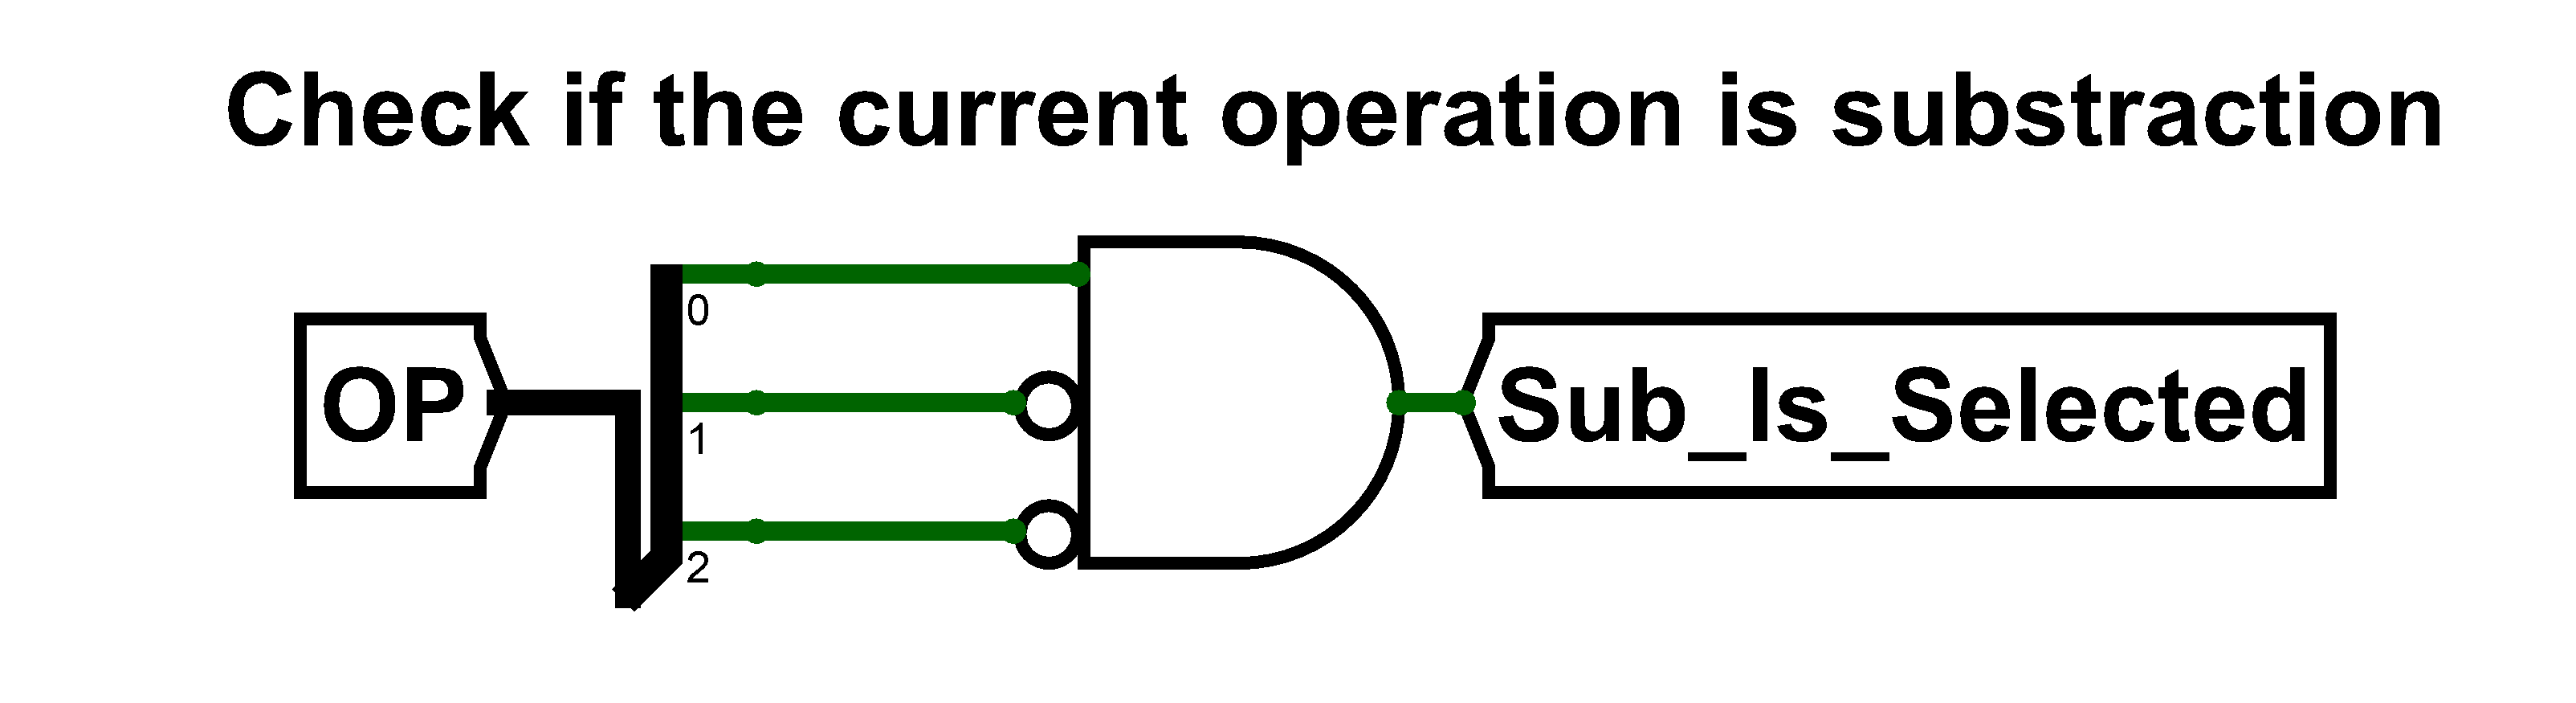
\includegraphics[width=.6\textwidth]{circuits/SubCheck.png}
     \caption{OP = 1 Checker}
 \end{figure}

 Given this information, we can decide whether we have to inverse the $B$ sign or not, we can use a 2 to 1 multiplexer for this.

  \begin{figure}[H]
     \centering
     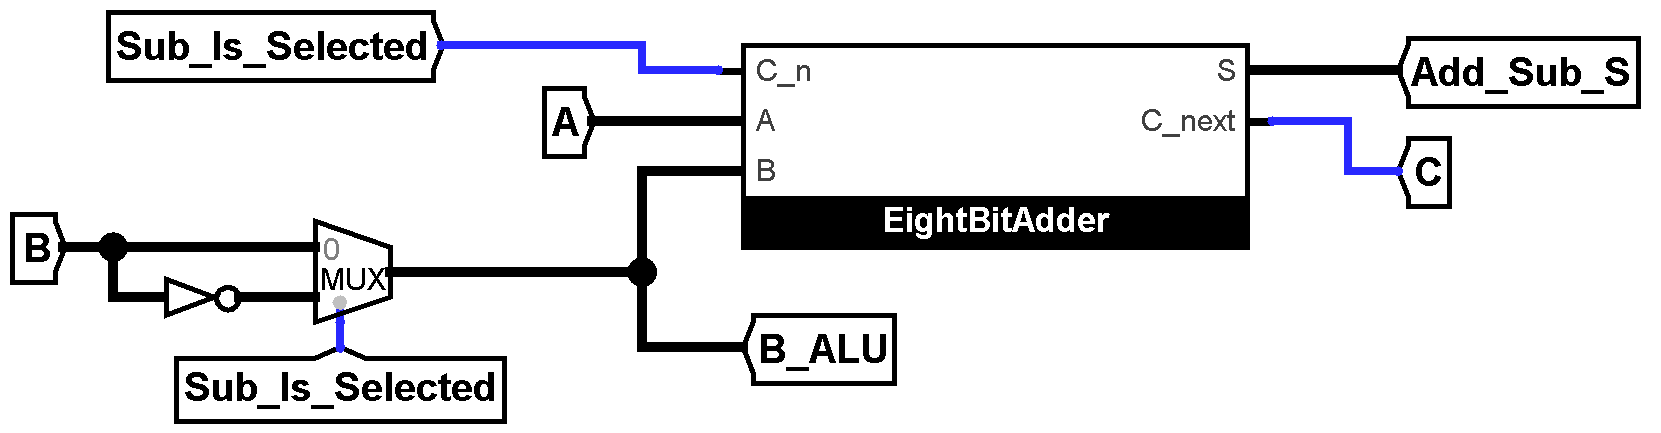
\includegraphics[width=.8\textwidth]{circuits/AdderSubtractor.png}
     \caption{ALU Adder/Subtractor}
     \label{fig:add_sub}
 \end{figure}

 We add a Tunnel at the output of the multiplexer to get the value of $B$ depending on the selected operation, this will come in handy later on when we implement the Status output.


\subsubsection{And, Or, Not, XOR}

Implementing these operations is very easy since Logisim already provides us with plug-and-play components that do the exact tasks, we only need to change the data size from a single bit to 8 bits.

\begin{figure}[H]
  \begin{subfigure}{0.5\textwidth}
    \centering
    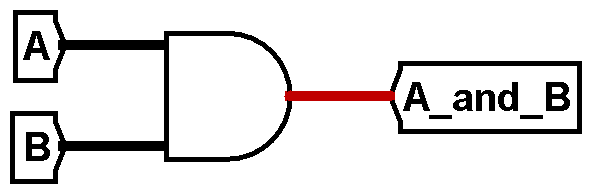
\includegraphics[width=0.8\linewidth]{circuits/and.png}
    \caption{And}
  \end{subfigure}%
  \begin{subfigure}{0.5\textwidth}
    \centering
    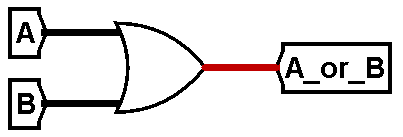
\includegraphics[width=0.8\linewidth]{circuits/or.png}
    \caption{Or}
  \end{subfigure}

  \begin{subfigure}{0.5\textwidth}
    \centering
    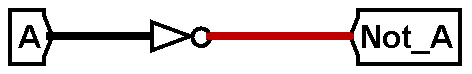
\includegraphics[width=0.8\linewidth]{circuits/not.png}
    \caption{Not}
  \end{subfigure}%
  \begin{subfigure}{0.5\textwidth}
    \centering
    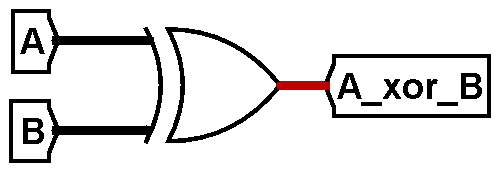
\includegraphics[width=0.8\linewidth]{circuits/xor.png}
    \caption{XOR}
  \end{subfigure}

  \caption{ALU Bit-by-Bit Operations}
\end{figure}

\subsubsection{Left and Right Shifting}

Logisim already provides us with Left and Right shift components that we use directly, however, given our $A$ and $B$ inputs are 8 bits each, the maximum value that we can shift is 7, beyond that, we would only get 0s, which is useless, so we should limit the input of $B$ from 255 to 7, by only taking the first 3 bits ($B_2$, $B_1$, and $B_0$).

We can achieve that with the build-in Splitter, by setting the Fan Out to 3 and the Bit In Width to 8, which will do $\lceil 8/3 \rceil = 3 $, and outputting bits 0 to 2 in the first output, 3 to 5 in the second, and the remaining 6 and 7 in the third. We then take the first output as our shifting amount.
\\[12pt]

\begin{figure}[H]
  \centering
  \begin{subfigure}{.5\textwidth}
    \centering
    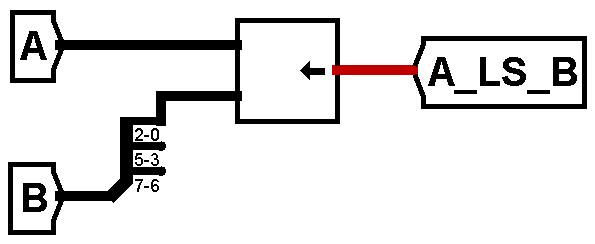
\includegraphics[width=0.8\linewidth]{circuits/leftshift.png}
    \caption{Left Shift}
  \end{subfigure}
  \\[24pt]
  \begin{subfigure}{.5\textwidth}
    \centering
    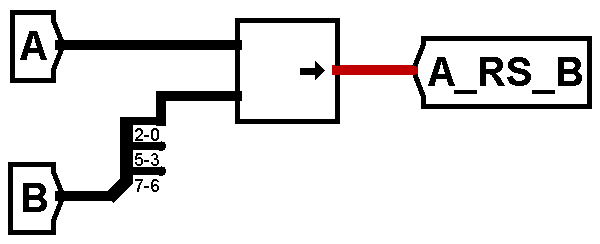
\includegraphics[width=0.8\linewidth]{circuits/rightshift.png}
    \caption{Right Shift}
  \end{subfigure}

  \caption{ALU shifting Operations}
\end{figure}


\subsection{Status}
Our ALU also has a 4-bit output as Status, each bit is a flag for a specific status of our result, mapped as follows:

\begin{enumerate}[start=0, before=\small, after=\normalsize, itemsep=2pt, parsep=0pt]
    \item \textbf{N}egative
    \item \textbf{Z}ero
    \item o\textbf{V}erflow: the result is not correct with
signed numbers, i.e. the sum of 2 positive numbers is a negative number.
    \item \textbf{C}arry: the result is not correct with unsigned numbers: this is the 9th bit of an
operation.
\end{enumerate}

We can use a Splitter in reverse to transform the single flags into a single 4-bit Status BUS.

\begin{figure}[H]
    \centering
    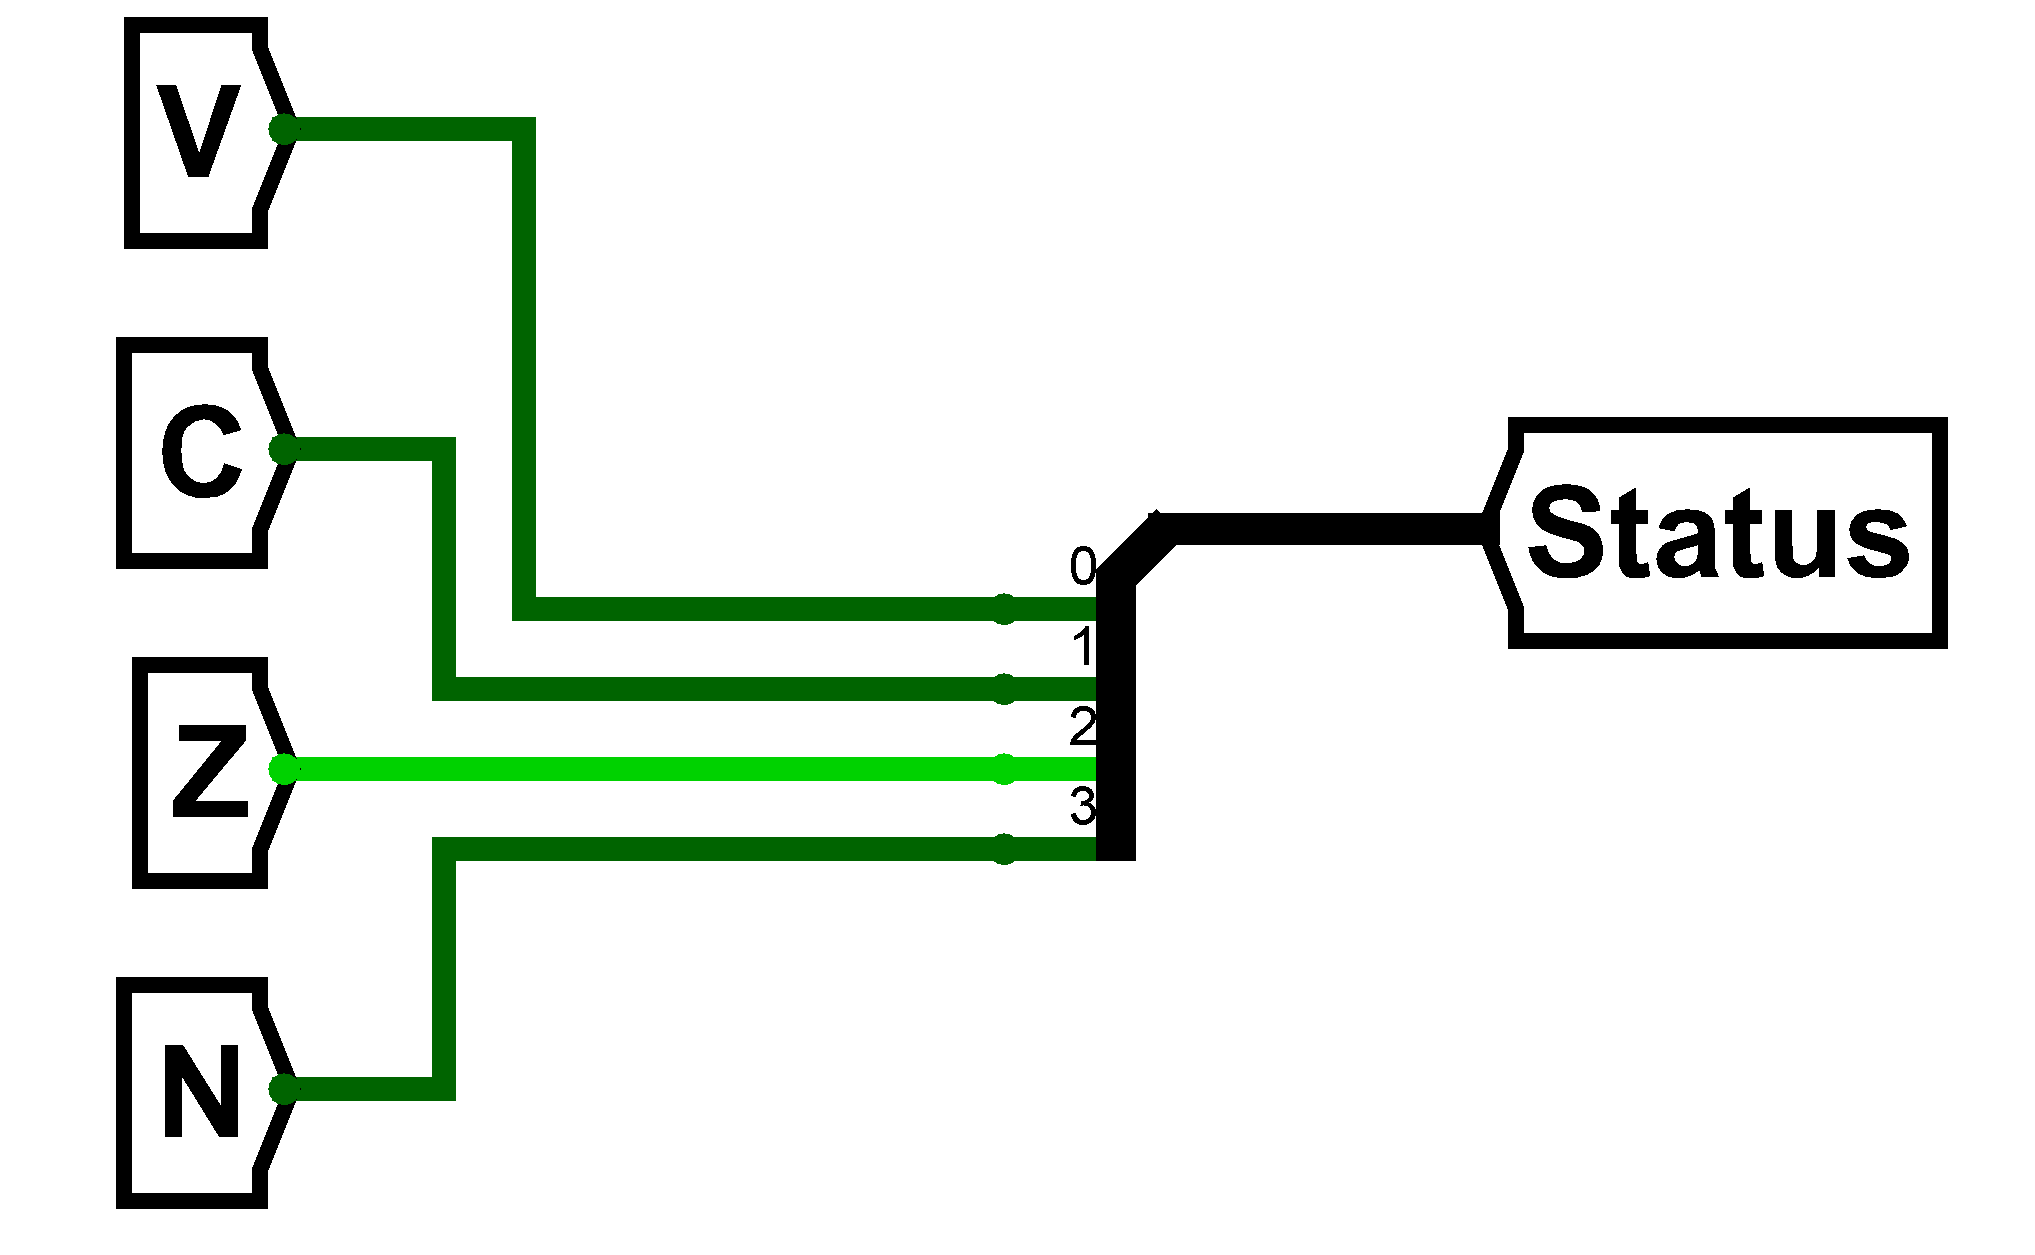
\includegraphics[width=.5\textwidth]{circuits/status_bus.png}
    \caption{ALU Status: BUS}
\end{figure}

\subsubsection{Negative}
This bit is straightforward to extract. Since we are using 2's complement to represent negative values, we can just check the MSB of our ALU output if it is equal to 1 or 0, 1 being negative, and positive otherwise. \\
We can use a splitter for the bit extraction.

\begin{figure}[H]
    \centering
    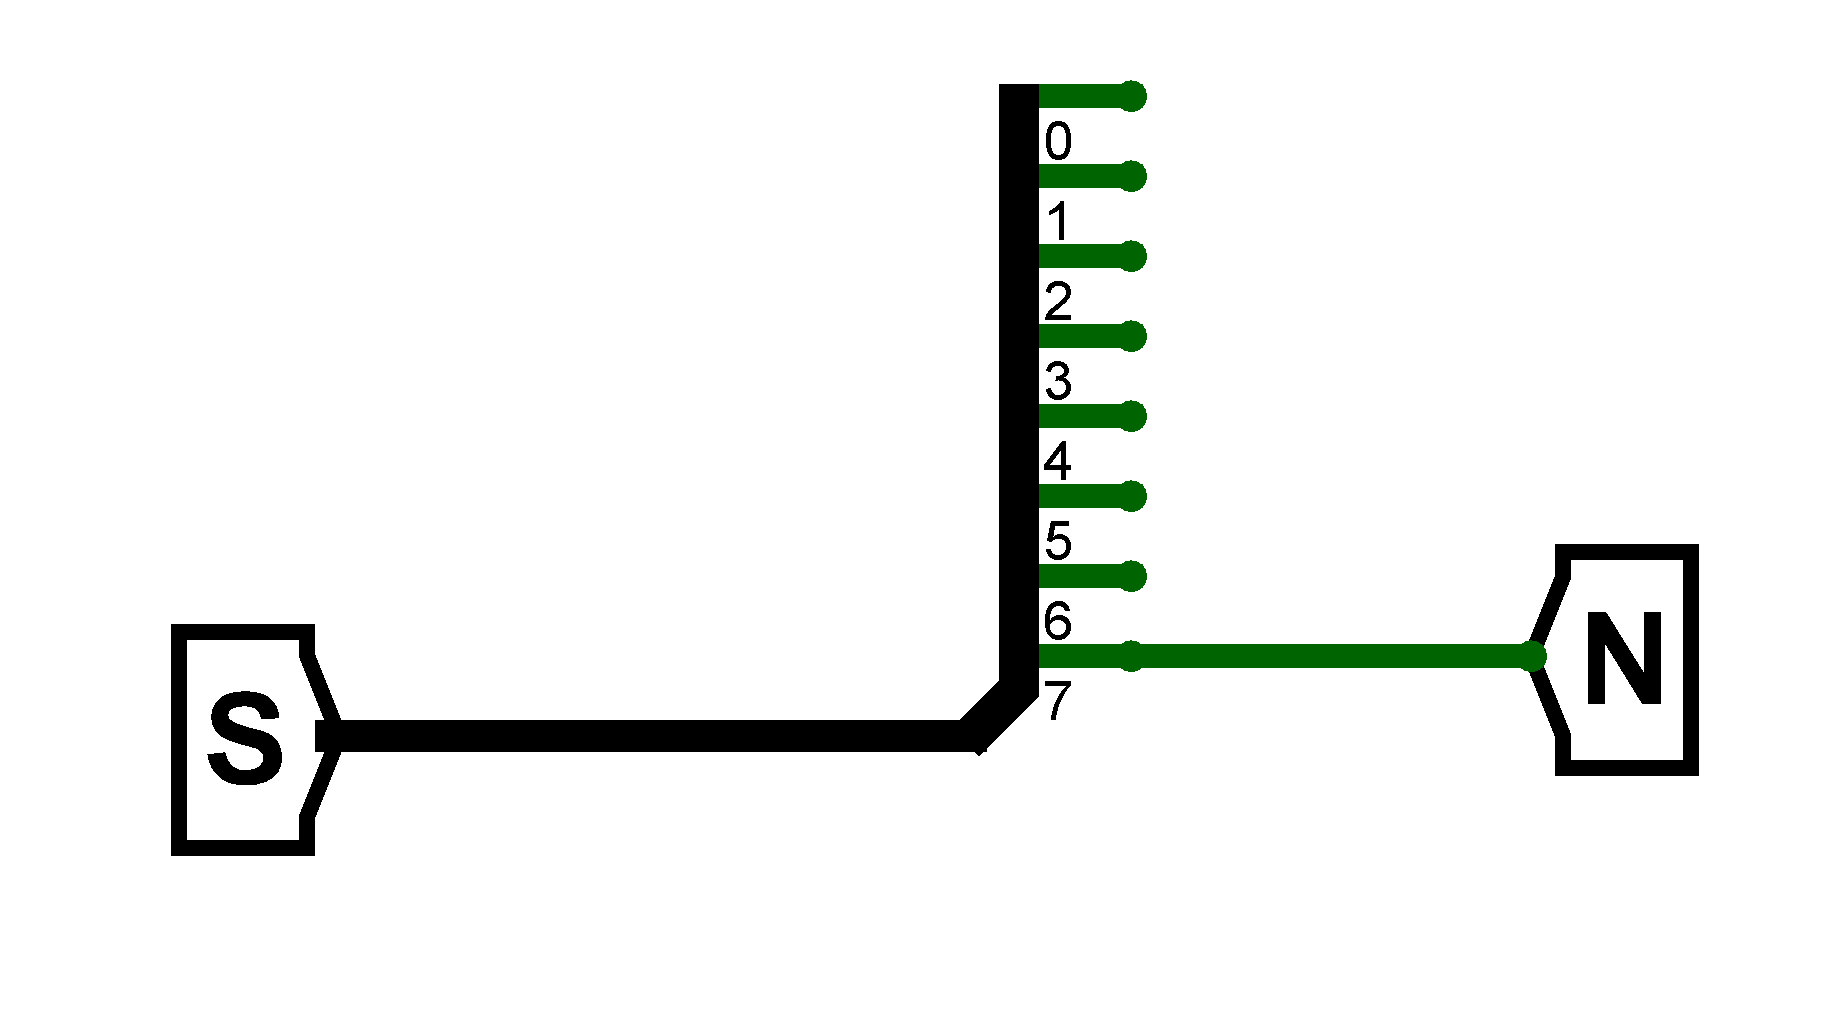
\includegraphics[width=.5\textwidth]{circuits/status_n.png}
    \caption{ALU Status: N Flag}
\end{figure}

\subsubsection{Zero}
We can find the Z flag by checking that every bit of our ALU output is equal to 0, giving us the following equation:
$$
Z = \overline{S_7} \cdot \overline{S_6} \cdot \overline{S_5} \cdot \overline{S_4} \cdot \overline{S_3} \cdot \overline{S_2} \cdot \overline{S_1} \cdot \overline{S_0} \; = \; \overline{S_7 + S_6 + S_5 + S_4 + S_3 + S_2 + S_1 + S_0}
$$
We can implement the second equation with a single 8-input NOR gate.

\begin{figure}[H]
    \centering
    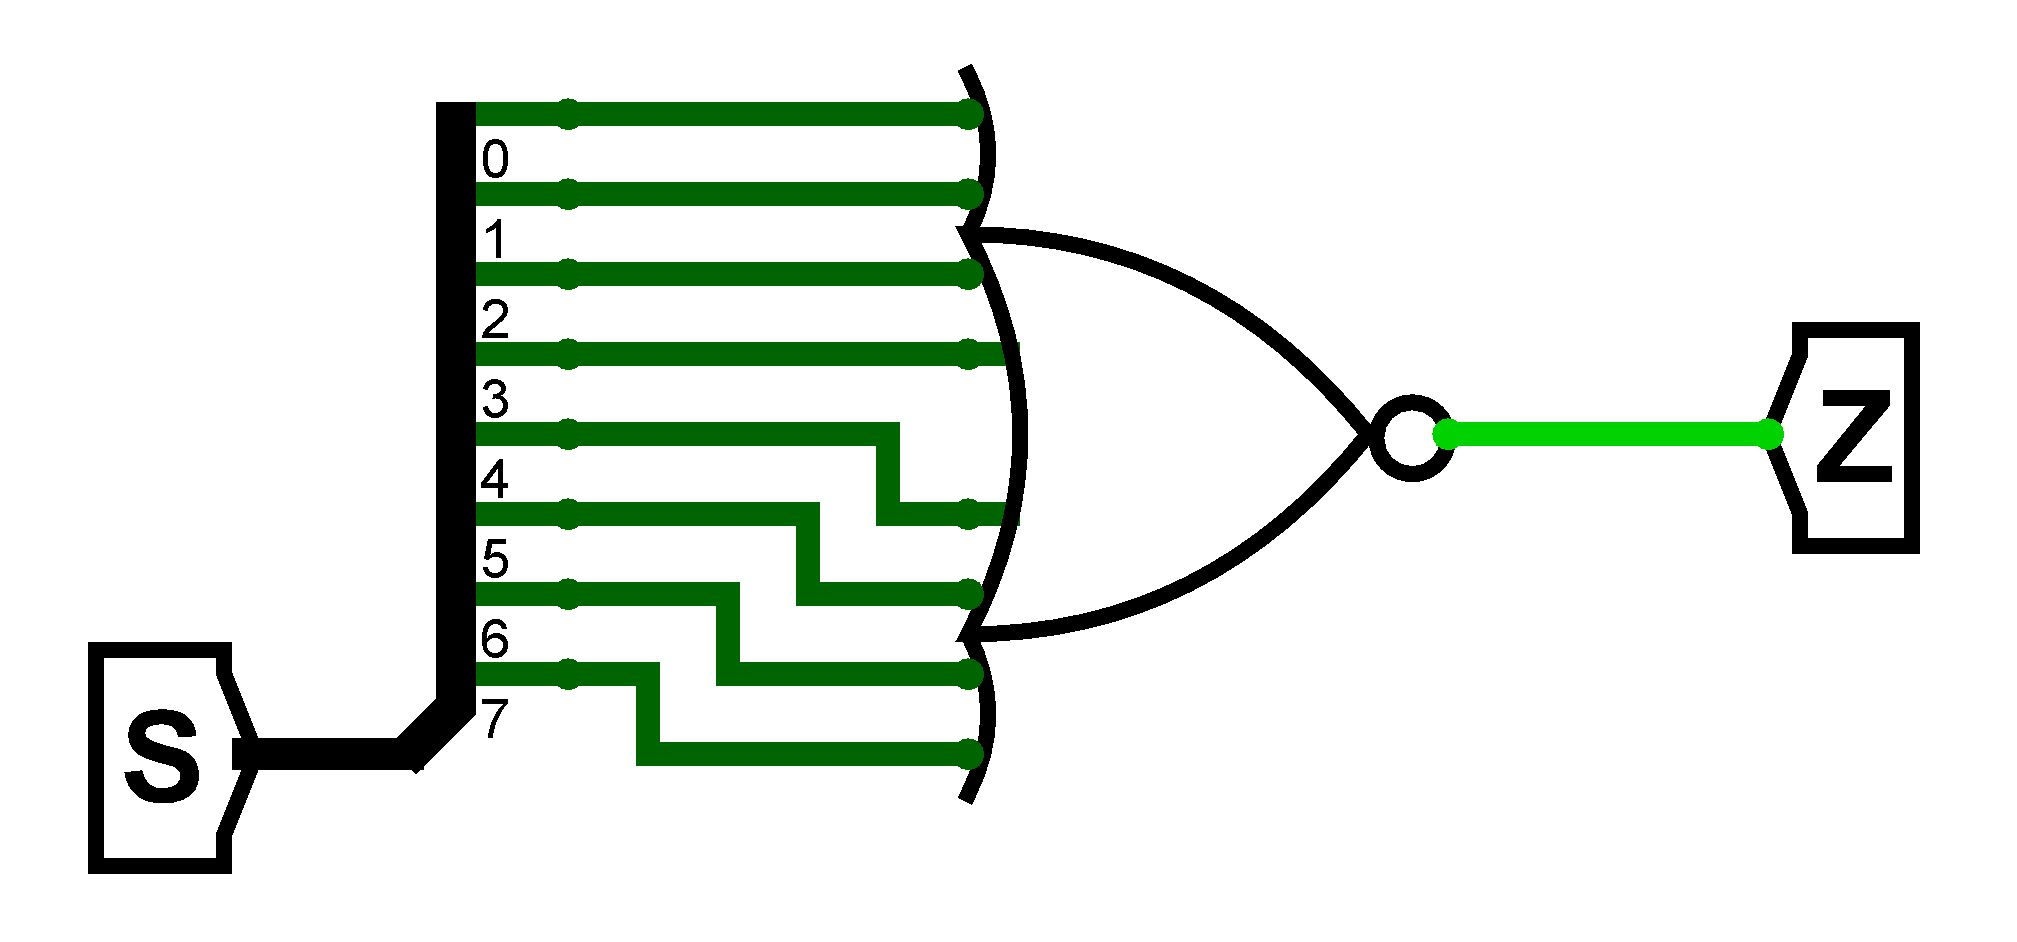
\includegraphics[width=.5\textwidth]{circuits/status_z.png}
    \caption{ALU Status: Z Flag}
\end{figure}

\subsubsection{oVerflow}
As explained above, the oVerflow Flag is set when the result of addition or subtraction overflows into the sign bit (MSB), which renders the result incorrect.

If the result of an addition between two positive numbers is negative (MSB of S is 1) we know that we have an overflow, similarly, if the addition of two negative numbers is positive (MSB of S is 0) we know that there is an overflow.
This also applies if A + B if both A and B are negative, or A - B if B is negative.

This can be irritating to implement for all use-cases, but we can heavily simplify our check if we take the B from the multiplexer that we have already set up in our Adder/Subtractor, this will take care of all the use-cases, and the only thing remaining is to check if the sign of A and B is coherent with the sign of the result S (the N flag previously implemented).

$$
V = MSB(A) \cdot MSB(B) \cdot \overline{N} + \overline{MSB(A)} \cdot \overline{MSB(B)} \cdot N
$$

\begin{figure}[H]
    \centering
    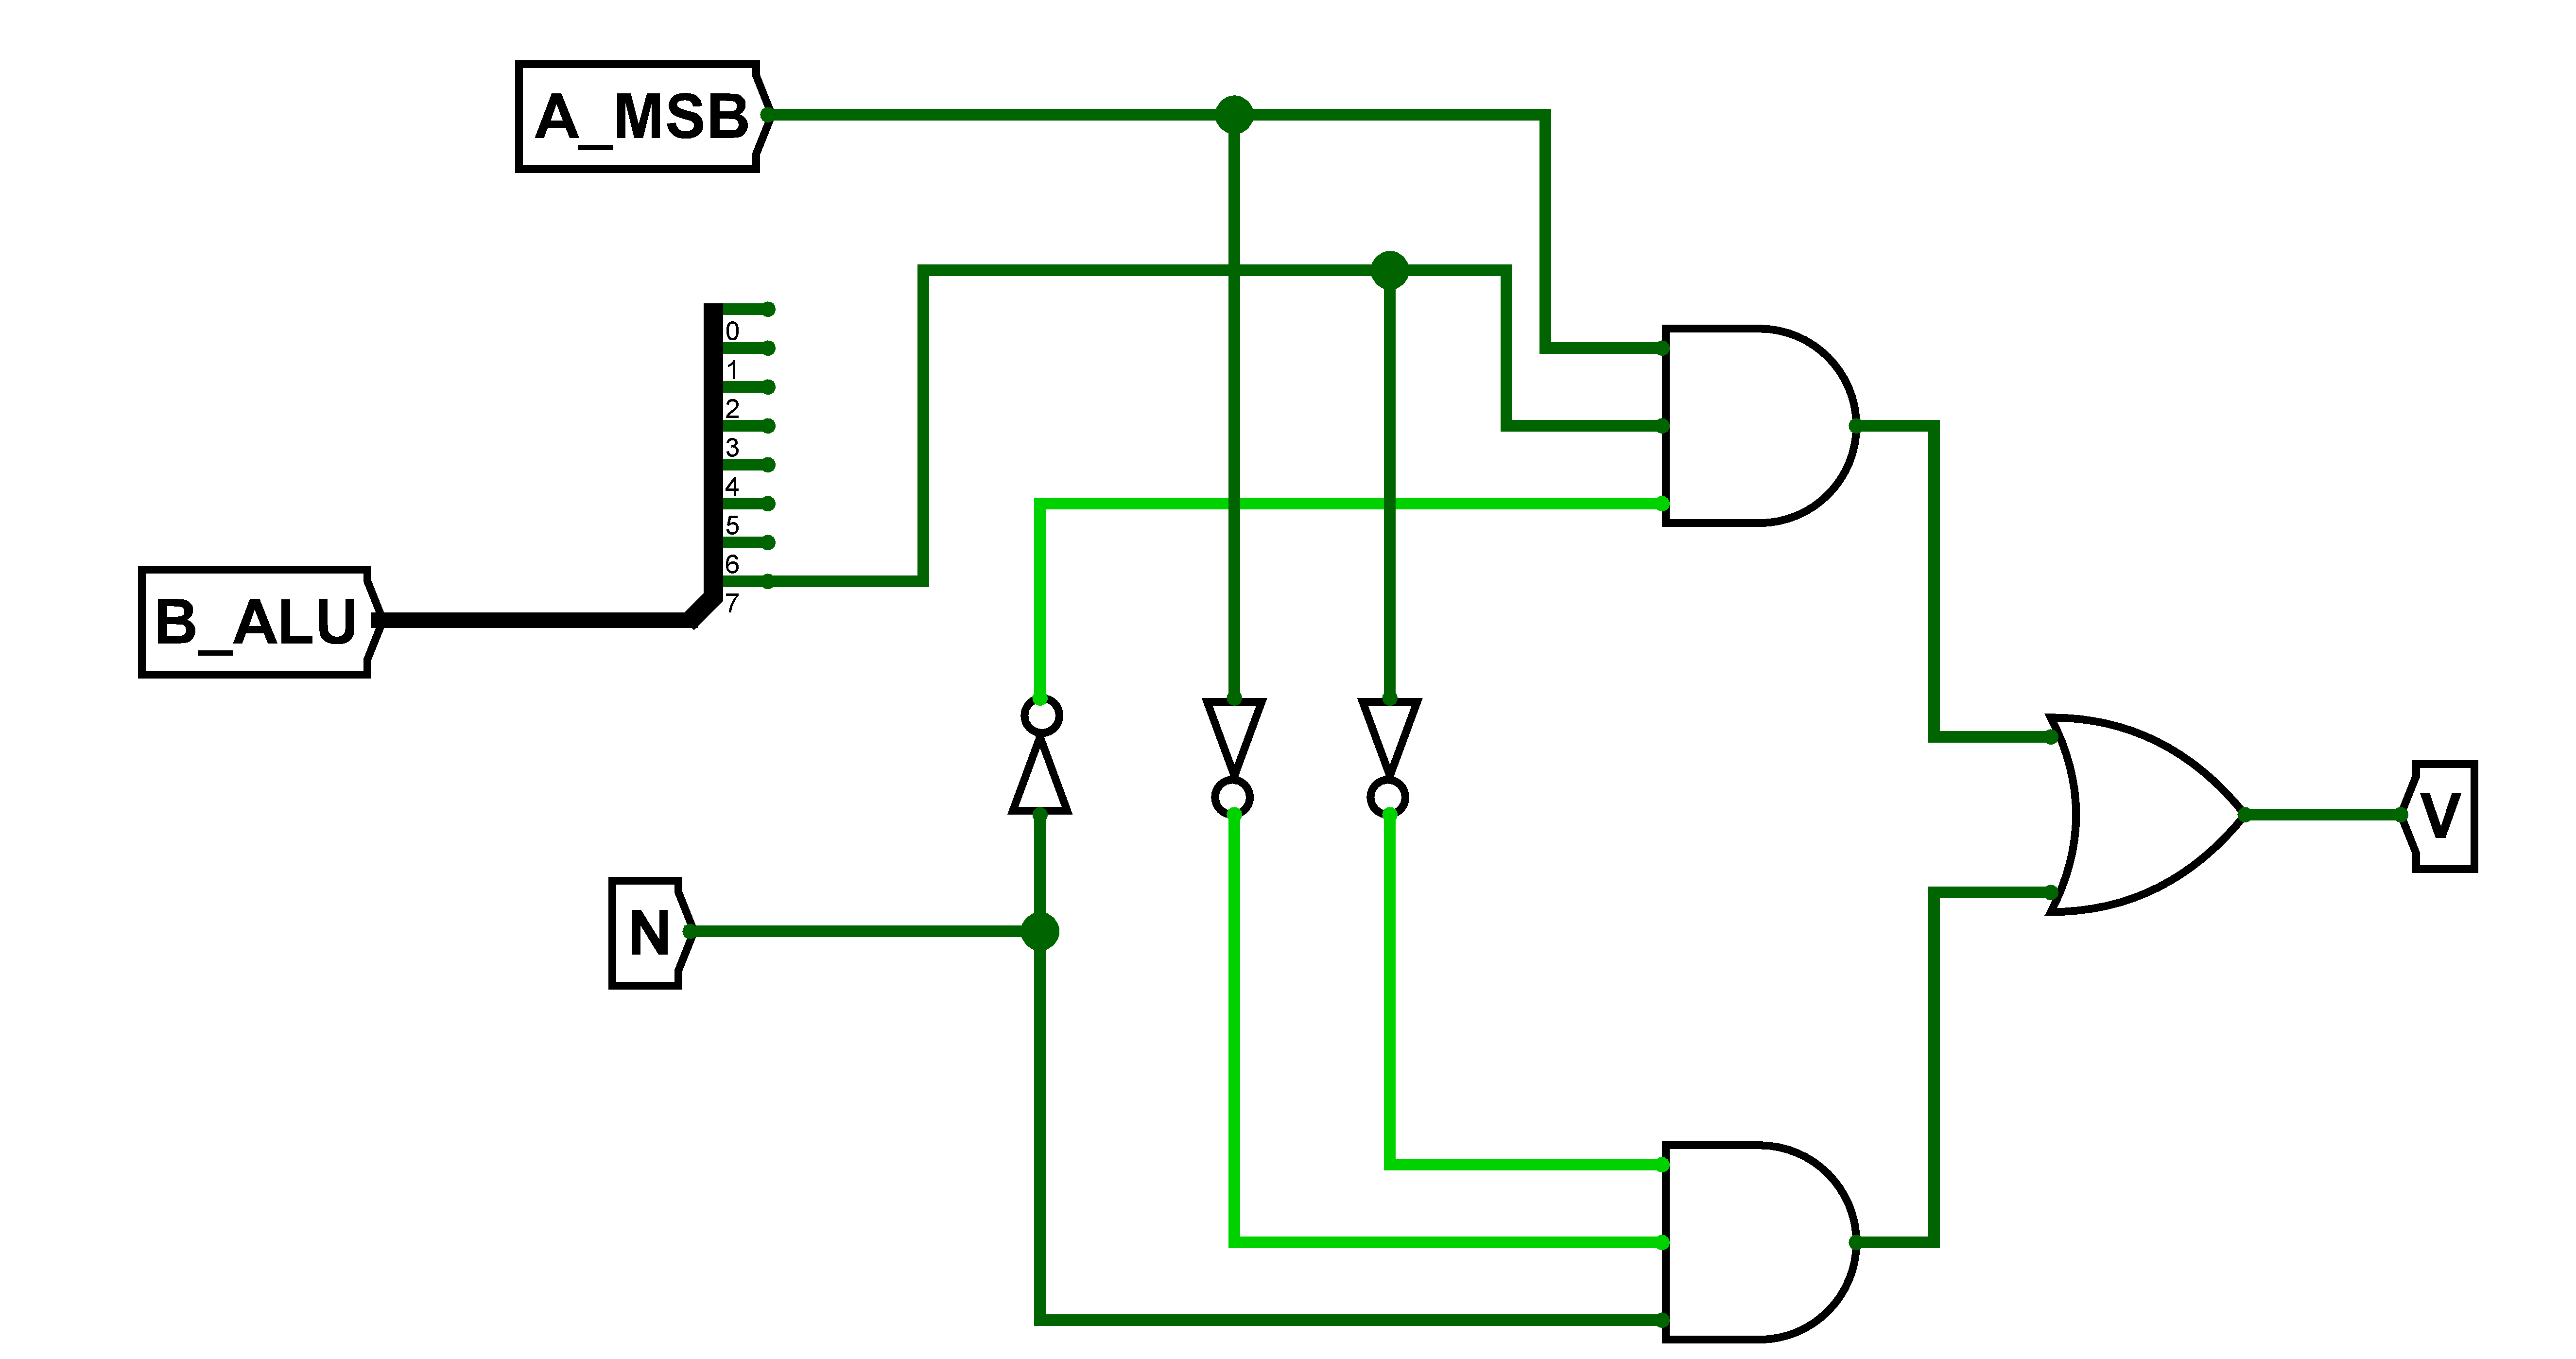
\includegraphics[width=.8\textwidth]{circuits/status_v.png}
    \caption{ALU Status: V Flag}
\end{figure}

\subsubsection{Carry}

Similar to the N flag, this is straightforward to find, it is equal to $C_n$ of our Adder/Subtractor. (See Figure \ref{fig:add_sub})

\subsection{One Step Further!}

\subsubsection{Arithmetic right shift}
An arithmetic right shifter is an ordinary right shifter, but it is sign-aware!!. \\
If the input is negative (MSB is 1), instead of filling the gap with 0s, it will fill it with 1s instead, keeping the same sign of the result.

We think our solution is not the best, or the most efficient. We have simply extended the $A$ input from 8 bits to 16 bits. the extra 8 bits are either 0s (0x00) if $A$ is positive, or 1s (0xFF) if $A$ is negative. With this in mind, we have to also extend the shifting amount to be coded on 4 bits instead of the previous 3 ($16 = 2^4$), so we just forced the $3^{rd}$ bit to always be 0 by hooking it to ground.

\begin{figure}[H]
    \centering
    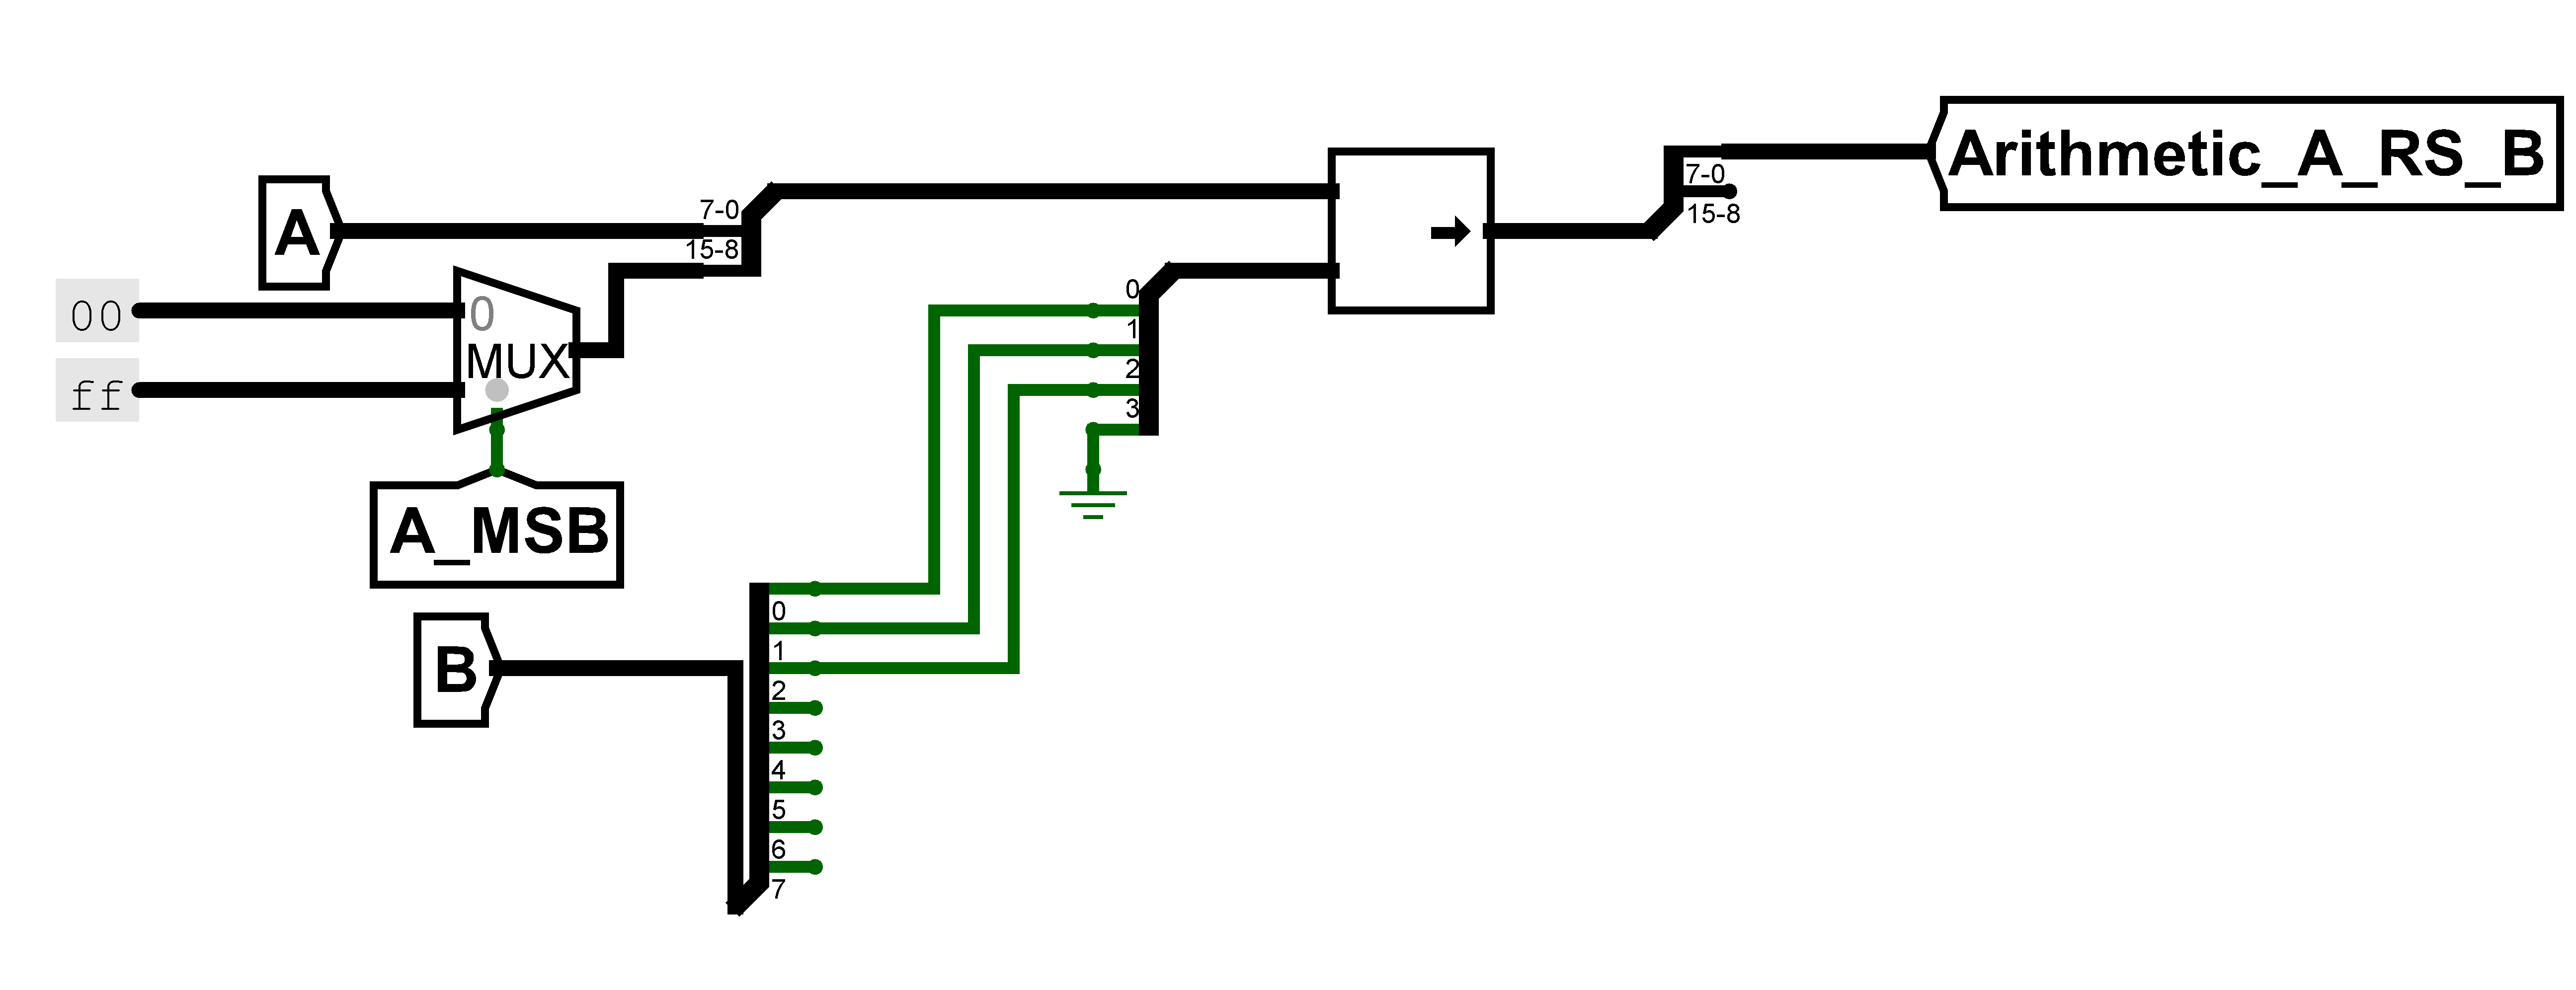
\includegraphics[width=\textwidth]{circuits/arithmeitc_rs.png}
    \caption{Arithmetic Right Shift}
\end{figure}

\section{Conclusion}
In conclusion, the successful implementation of an 8-bit Arithmetic Logic Unit (ALU) in Logisim has provided us with valuable hands-on experience in digital logic design. This project allowed us to apply our knowledge of combinational circuits, logical operations, and circuit simulation to create a functional ALU that can perform a variety of arithmetic and logic operations. \\
We would have loved it if we were able to implement the Multiplier circuit, but unfortunately, due to its complexity, our humble knowledge, and the limited time we had (traveling to different cities where our companies are), we couldn't find enough time to understand and implement the circuit. \\
Nevertheless, through this project, we gained a deeper understanding of the complexities and intricacies of digital circuits and the importance of careful design and testing. Overall, our work on the 8-bit ALU in Logisim has been an insightful and rewarding journey into the world of digital design.

\section*{Resources}
\addcontentsline{toc}{section}{Resources}
The Logisim Circuit File, and this report's source code, are available on this GitHub repository: \href{https://github.com/elkhayder/sec1-tp-mac}{elkhayder/sec1-tp-mac} 

\end{document}
